
%%******************************************************************************
%% SECTION - Resultados alcançados (resumo de medidas efetuadas, resultados de análises e ensaios, especificações de protótipos, etc.);
%%******************************************************************************
\setcounter{secnumdepth}{3}
\section{Resultados Alcançados}
\label{resultados_alcancados}

\subsection{Eletrônica:}

A partir da primeira solução conceitual para a eletrônica, foram projetadas duas PCBs, seus projetos conceituais, esquemáticos e modelos 3D com roteamento (a ferramenta utilizada foi o software Altium). Uma placa tem como objetivo garantir robustez através de redundância de micro controladores, enquanto que a outra foca em simplicidade, entrega rápida e de menor custo. Alguns componentes da placa já estão disponíveis em laboratório e foram testados, outros estão na lista de componentes que serão adquiridos ainda até fim de maio.
A segunda solução para a eletrônica embarcada, que envolve a utilização de um PC, resultou na pesquisa de fornecedores de PC104 com placas ADC e CAN. Drivers de diversos dispositivos já estão disponíveis em ROCK, o que facilita a execução desta solução tanto para software quanto para hardware.  
Por último, em Maio, foi montada uma eletrônica embarcada protótipo para os testes em Jirau. Serão utilizadas as interfaces RS232-USB e analógica para os testes do sonar Micron (disponível em laboratório) e sensores indutivos. A alimentação será realizado por um pack de baterias 12V, 7Ah em série. A proposta de soluções para a arquitetura da eletrônica do projeto ROSA encontra-se no Relatório de Eletrônica. 

 \begin{figure}[ht!]
    \centering 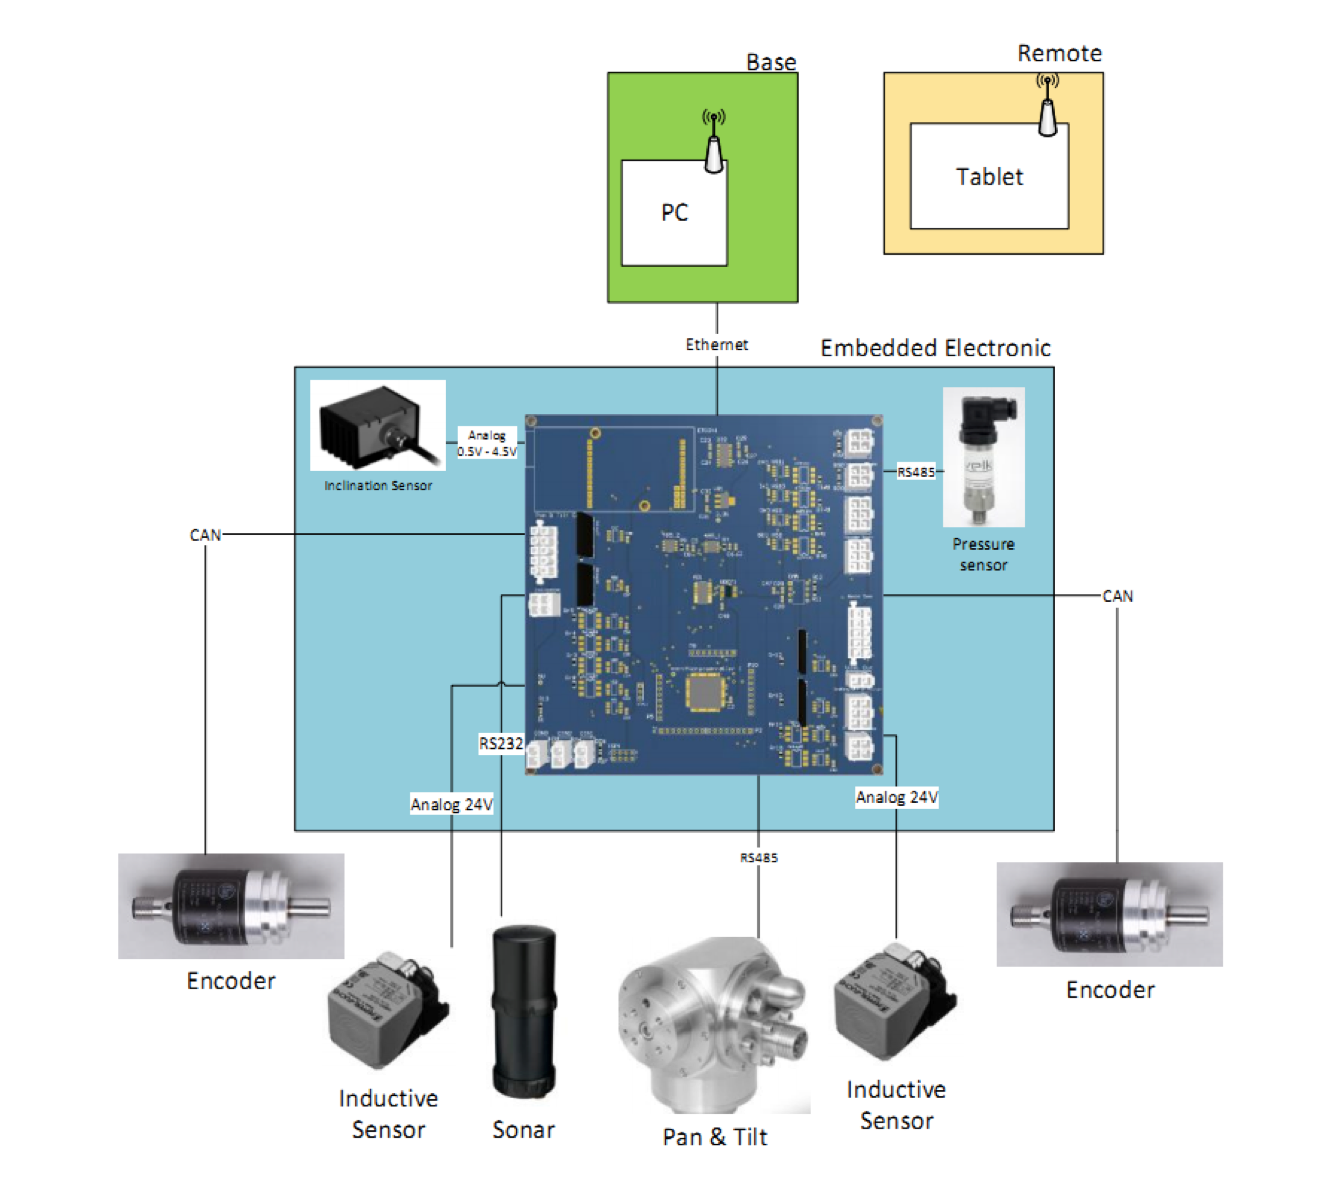
\includegraphics[width=1\columnwidth]{figs/resultados/eletronica}
    \caption{Diagrama de Eletrônica}
    \label{fig:eletronica}
\end{figure}


\noindent
\subsection{Reconstrução 3D por Sonar}

O princípio por trás da parte reconstrução 3D do projeto é  acumular os dados volumétricos provenientes do sonar em uma representação volumétrica. Esse acúmulo ajuda a resolver o problema de ambiguidade dos dados de sonar. O framework Octomap foi definido durante a fase de definição do projeto como a biblioteca a ser utilizada para o acúmulo volumétrico. Logo, o Octomap foi integrado ao framework Robot Construction Kit (ROCK), framework de robótica utilizado no projeto. A integração foi testada em laboratório utilizando-se um sonar Tritech Micron, a figura \ref{fig:octomap} demonstra o preenchimento volumétrico de preenchendo o mesmo de acordo com a forma de onda proveniente do sonar e a intensidade de reflexão. 

\begin{figure}[ht!]
    \centering 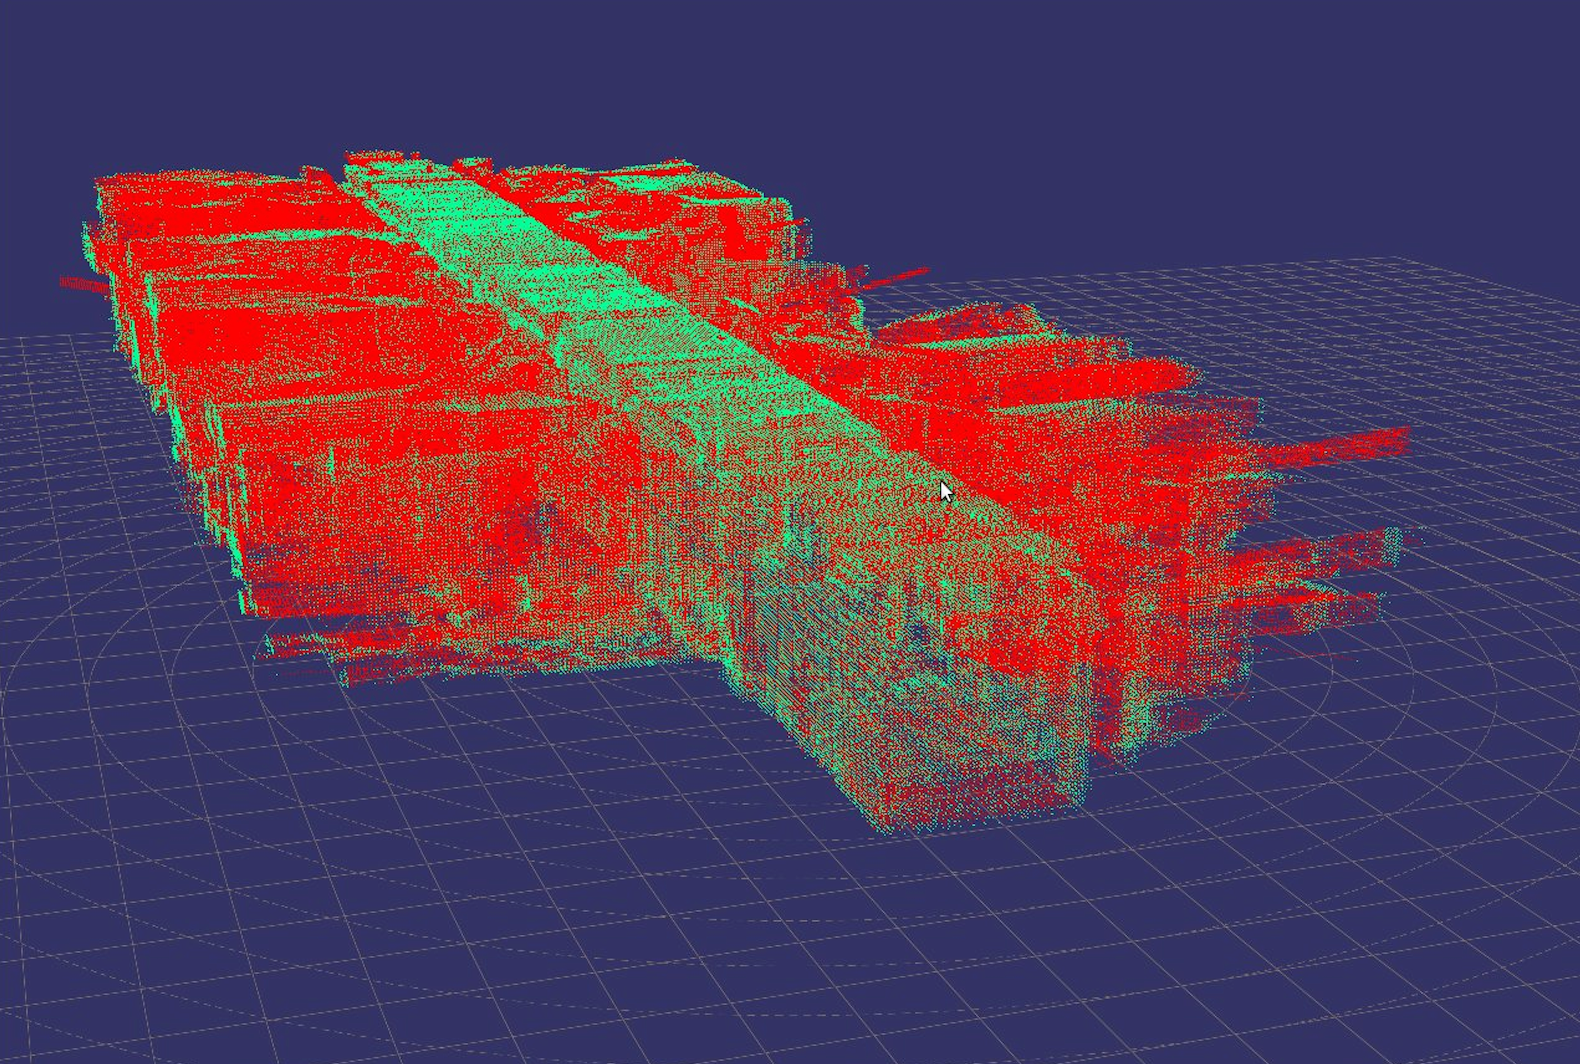
\includegraphics[width=1\columnwidth]{figs/resultados/octomap}
    \caption{Octomap}
    \label{fig:octomap}
\end{figure}

\noindent
\subsection{Interface}

A interface de usuário facilita a utilização do robô ROSA, permitindo a compreensão das informações geradas pelo robô de modo intuitivo. 
No quadrimestre o protótipo da interface foi desenvolvido e implementado em um tablet Android para análise de usabilidade, \ref{fig:userinterface}.   
A prototipagem é uma técnica de análise iterativo em que os usuários estão ativamente envolvidos no desenvolvimento da interface. 
A descrição detalhada do protótipo de interface encontra-se no Relatrório de Interface de Usuário.

\begin{figure}[ht!]
    \centering 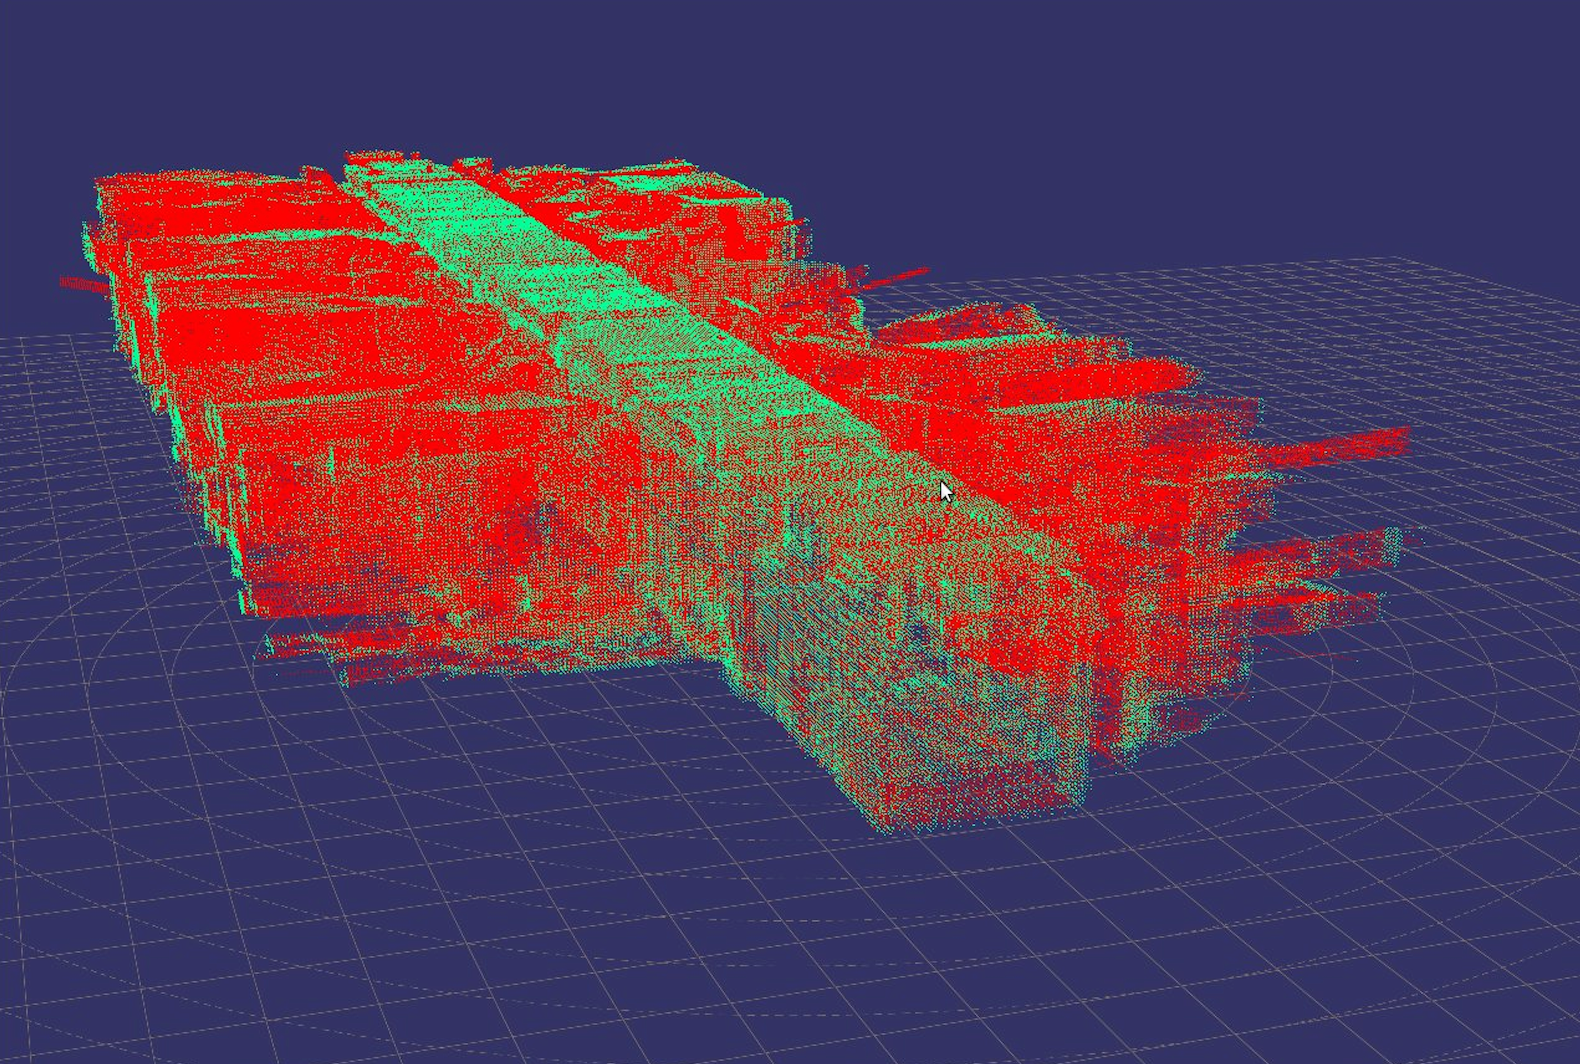
\includegraphics[width=1\columnwidth]{figs/resultados/octomap}
    \caption{Interface Usuário}
    \label{fig:userinterface}
\end{figure}

\noindent
\subsection{Drivers}
Os drivers permitem a comunicação entre o computador e os hardwares ou dispositivos conectados ao mesmo. 
No quadrimestre foram comprados os sensores especificados no projeto básico, dentre os sensores comprados o sensor indutivo, encoder e profundimetro foram entregues. 
Os drivers para os dispositivos entregues foram desenvolvidos, integrando os mesmos ao Framework de robótica ROCK. 
A comunicação e funcionalidade dos dispositivos foram testados em bancada.




  